\hypertarget{sec:evaluation}{%
\chapter{Evaluation}\label{sec:evaluation}}

This chapter evaluates the \gls{awsm} approach according to the requirements stated in \cref{sec:requirements}.
This assessment is followed by a comparison to the state of the art in terms of benefits and weaknesses.
Finally, the application of \gls{awsm} in the context of the thesis scenario is outlined.

\vspace{-15pt}
\hypertarget{requirements-evaluation}{%
\section{Requirements Evaluation}\label{requirements-evaluation}}
\vspace{15pt}

In the following, the \gls{awsm} approach is assessed with regard to the scope and stakeholder requirements of this thesis.
To conduct this evaluation, each requirement is considered separately against the solutions provided by the \gls{awsm} Methodology and their support through the Toolsuite.
The same criteria that were used for the assessment of the state of the art of \gls{Web Migration} approaches in \cref{sec:approaches} are applied to \gls{awsm}.
Where applicable, the assessment of requirements refers to the experimentation results presented for each \gls{awsm} Method and its corresponding Tools in order to further support the assessment.

\vspace{-10pt}
\hypertarget{sec:evaluation.scope-requirements}{%
\subsection{Scope Requirements}\label{sec:evaluation.scope-requirements}}
\vspace{10pt}

The following scope requirements are evaluated to determine to what extent \gls{awsm} address the scope set in \cref{sec:scope}, i.e.~to what extent it is a \gls{Web Migration} approach supporting the initial phase of a \gls{Web Migration} and having \glspl{Web Application} as target architecture.

\subsubsection*{S1 Initial Phase Support}
The Methodology and Toolsuite provided by \gls{awsm} dedicatedly addresses the initial phase of \gls{Web Migration} prior to actual \gls{Transformation} and beyond knowledge recovery.
\Cref{tbl:awsm-remip} presented a mapping of \gls{awsm} Methods onto the phases of the \gls{remip} reference model, placing AWSM:RE and AWSM:RM in the first phase.
While AWSM:RE focuses on knowledge recovery, AWSM:RM goes beyond this.
The \gls{risk management} method based on \gls{Rapid Web Migration Prototyping} specifies a set of activities that are to be executed even before the final decision whether to migrate to the \gls{web} or not has been made.
In this early pre-migration phase, AWSM:RM addresses the communication of necessity and benefits of a \gls{Web Migration} through transfer of the \gls{Rapid Prototyping} paradigm into the \gls{Web Migration} domain.
In this way, the AWSM:RM method and \gls{rewamp}/\gls{rwmpa} and UI Transformer toolchain facilitate the creation of \glspl{web migration prototype} as concrete, tangible demonstrative products contributing to making the migration \gls{business case} and as a vehicle for communication across stakeholders serving as a basis for decision making.
Furthermore, the \gls{s2dcs} Tool presented in \cref{sec:s2dcs} facilitates \gls{Web Migration} strategy selection, an essential activity in the initial phase, based on data from a systematic mapping study comprising scientific publications and software tools.
According to the assessment scheme, the requirement is fully satisfied.

\vspace{-10pt}
\subsubsection*{S2 Web Application Target}
The \gls{awsm} Methodology and Toolsuite has \glspl{Web Application} according to \cref{def:webapplication} as target architecture.
\gls{awsm} \glspl{target system} are \glspl{Web System}, communicating via \gls{http} and based on \gls{w3c} standards like \gls{html}, \gls{css}, \gls{wasm}, that provide content and services through a \glslink{web}{Web}-based user interface.
This can be seen in the architecture of AWSM:RM prototypes presented in \cref{fig:awsm.rm.overview} and the comparative analysis of \web user interfaces and their corresponding \legacy versions enabled through AWSM:CI as presented in \cref{sec:visual-analysis}.
The target \glslink{web}{Web}-based user interfaces created through AWSM:RM are not mere wrappers, but real \glspl{wui}, implemented in \gls{html}, \gls{css}, JS, and are run independently of their \glslink{Legacy System}{legacy} counterparts.
They feature essential \gls{web} paradigms, like asynchronous request-response communication, spatial and technological client-server separation, and URL-based navigation of resources.
As \glspl{Web Application} are created based on existing non-\glslink{web}{Web} \glspl{Legacy System} in \gls{Web Migration}, AWSM:CI does support joint analysis of non-\glslink{web}{Web} and \glslink{web}{Web}-based user interface through a computer-vision based approach operating on visual features at a cross-platform level of abstraction, enabling consideration of target \glspl{Web Application} concerning \gls{ui} similarity with their \glslink{Legacy System}{legacy} counterparts.
Furthermore, also the tools of the \gls{awsm} Toolsuite itself are implemented based on open \gls{web} standards as reasoned in the design decision of principle \cref{p:1}.
According to the assessment scheme, the requirement is fully satisfied.

\vspace{-15pt}
\hypertarget{sec:evaluation.stakeholder-requirements}{%
\subsection{Stakeholder Requirements}\label{sec:evaluation.stakeholder-requirements}}
\vspace{5pt}

The following stakeholder requirements are evaluated to assess appropriateness of the \gls{awsm} Methodology and Toolsuite for the characteristics of an independent software vendor, as detailed in \cref{sec:scenario}.

\vspace{-10pt}
\subsubsection*{C1 Risk Management}
The \gls{awsm} Methodology and Toolsuite provide \gls{risk management} methods beyond basic feasibility-centric approaches through its AWSM:RE and AWSM:RM methods.
AWSM:RE enables a concept-assignment-based knowledge recovery approach, which addresses the risk of losing knowledge implicitly represented by the \glslink{Legacy System}{legacy} source code during \gls{Web Migration} (cf. \cref{sec:awsm-re}).
The systematic application of AWSM:RE \gls{Reverse Engineering} extracts knowledge from the source code and sustains it for further management and usage in an interoperable way based on the \gls{sckm} formalism and a queryable \gls{web} standards-based knowledge representation.
The experiment in \cref{sec:re.evaluation} has shown that \glspl{isv} are enabled to conduct this activity through crowdsourcing.
Following \gls{awsm} principle \cref{p:4}, AWSM:RM specifies a rapid-prototyping-based method for creating demonstrative \glspl{web migration prototype} that allows for identification of migration process and migration result risks (cf. \cref{sec:awsm-rm}).
The produced \glspl{web migration prototype} and gained migration experience not only provide insights on the technical feasibility, but they also represent a concrete and tangible contribution towards the \gls{Web Migration} \gls{business case}: they allow assessing the plausibility and thus desirability of a potential \glslink{web}{Web}-based version of the \gls{Legacy System} which enables an informed balancing of potential business value and cost.
The experiments in \cref{sec:rm.evaluation} have shown that these \glspl{web migration prototype} can be created from base material of the existing \gls{Legacy System} enabled through the \gls{awsm} Tools for \gls{Rapid Web Migration Prototyping}.
According to the assessment scheme, the requirement is fully satisfied.
\vspace{-10pt}

\vspace{-10pt}
\subsubsection*{C2 Reuse of Legacy Assets}
The \gls{awsm} Methodology and Toolsuite addresses reuse of \glslink{Legacy System}{legacy} assets at three different levels, covering the conceptual model, view and controller layers of an application: AWSM:RE focuses on reuse on the model and requirement level, AWSM:RM on the business logic and \gls{ui} level and AWSM:CI on the view and user interaction level.
In this way, the three \gls{awsm} Methods establish continuity of functionality (AWSM:RE and AWSM:RM) and user interaction (AWSM:RM and AWSM:CI) across \glslink{Legacy System}{legacy} and target \gls{Web System}.
The reuse of \glslink{Legacy System}{legacy} models and requirements is achieved through AWSM:RE by reverse-engineering these assets implicitly represented in the codebase into explicit \glspl{artifact}, thus enabling their reuse in both model-driven and non-model-driven subsequent processing.
The reuse of business logic and the user interface is achieved through AWSM:RM by semi-automatic (\gls{rewamp}) / automatic (UI Transformer) \gls{Transformation} based on \glslink{Legacy System}{legacy} code \glspl{artifact}, as shown in the experiments in \cref{sec:rm.evaluation}.
The reuse of view layout and user interaction is achieved through AWSM:CI by enabling a joint analysis of \glslink{Legacy System}{legacy} and \gls{web} user interfaces based on corresponding user interface \glspl{artifact}.
The experiment in \cref{sec:ci.evaluation} has shown that the proposed similarity computations can act as approximations of perceived similarity, ensuring continuity between \legacy and \web user interfaces.
The \gls{kdm}-based \gls{Legacy System}, \gls{sckm}, and Legacy User Interface formalisms provide the conceptual foundation of reuse in \gls{awsm}.
According to the assessment scheme, the requirement is fully satisfied.

\vspace{-10pt}
\subsubsection*{C3 Expertise \& Tool Support}
The \gls{awsm} Methodology and Toolsuite address expertise and tool support requirements through a method design integrating the non-functional expertise requirement for all three \gls{awsm} Methods and the tools of the \gls{awsm} Toolsuite, respectively.
AWSM:RE addresses the expertise requirement by reusing program comprehension results from ongoing \gls{Forward Engineering} and by automatic decomposition of \gls{Concept Assignment} into microtasks solved using crowd expertise.
The experiment in \cref{sec:re.evaluation} has demonstrated that the crowd worker's expertise and results quality is sufficient to reduce effort and expertise requirements on \gls{isv} staff by outsourcing it to the crowd.
AWSM:RE tool support comprises the Annotation Platform, its CSRE extension, and the tools for integration with ongoing development.
AWSM:RM addresses the expertise requirement by enabling business logic reuse based on existing staff expertise in the \glslink{Legacy System}{legacy} platform supported by the \gls{rewamp} toolchain, lowering the required \gls{Web Engineering} and migration expertise demand through its semi-automatic process supported by the extensive \gls{rwmpa} guidance and avoiding \gls{Web Engineering} requirements for \gls{ui} creation through the fully automatic UI Transformer without manual interventions.
The experiments in \cref{sec:rm.evaluation} have demonstrated feasibility of AWSM:RM with limited migration and \gls{Web Engineering} expertise.
AWSM:CI addresses the expertise requirement by specifying calibratable similarity measures that can be computed and empirically adjusted by existing \gls{isv} staff with fundamental statistics expertise based on automated visual \gls{ui} Element detection and with non-expert test subjects form the target group as demonstrated by the experiment in \cref{sec:ci.evaluation}.
The \gls{awsm} Toolsuite provides tool support for all three \gls{awsm} Methods enabling semi-automatic or automatic processes, fulfilling the tool aspect of the requirement.
As \gls{awsm} cannot entirely avoid expertise demand in new areas but is still feasible with existing staff, the expertise aspect of the requirement is conditionally met.
Thus, the overall requirement is assessed as half satisfied, acknowledging that \gls{Web Migration} activities can hardly be conducted without any additional expertise requirements.

\vspace{-15pt}
\subsubsection*{C4 Agile Development Process Integration}
The \gls{awsm} Methodology and Toolsuite address development process integration through a method design specifying the conceptual integration of each \gls{awsm} method into ongoing development activities and the integration support tools of the \gls{awsm} Toolsuite.
\gls{awsm} principle \cref{p:2} avoids specification of a stand-alone process: the three \gls{awsm} Methods targeting the initial phase can be integrated easier than full-coverage \gls{Web Migration} approaches.
\gls{awsm} principle \cref{p:3} facilitates integration with a variety of different model-driven or non-model-driven development processes.
AWSM:RE integrates with ongoing development through continuous \gls{Reverse Engineering}, embedding \gls{Concept Assignment} with \gls{Forward Engineering} in the comprehension phase, reusing the mental representation.
This is supported by the \gls{ide} integration tool.
AWSM:RE integrates \gls{Web Migration} project management with software project management via the migration package/migration backlog formalism and the corresponding project management tool integration.
AWSM:RM integrates with ongoing development through transfer of the \gls{Rapid Prototyping} paradigm into the \gls{Web Migration} domain, embedding AWSM:RM activities with ongoing explorative or experimental \gls{Prototyping}, with resulting \glspl{web migration prototype} as product increments achievable within one Scrum sprint.
AWSM:CI integrates with ongoing development in the context of software quality measurements and user interface design activities within ongoing \gls{Forward Engineering} \gls{uix} analysis and approval activities of a dedicated team of \gls{uix} experts.
As \gls{awsm} specifies integration with ongoing development for all three methods but introduces activities and \glspl{artifact} that, depending on the maturity of the ongoing forward development process, can be new, the development process integration is conditionally met.
Thus, the overall requirement is assessed as half satisfied, acknowledging that \gls{Web Migration} activities can hardly be entirely integrated with ongoing forward development.

\Cref{tbl:AWSM-eval} shows the overall evaluation results of \gls{awsm}.

\hypertarget{tbl:AWSM-eval}{}
\begin{longtable}[]{@{}llllll@{}}
\caption{\label{tbl:AWSM-eval}AWSM Evaluation}\tabularnewline
\toprule
S1 Initial & S2 Web & C1 Risk & C2 Reuse & C3 Exp & C4 Agile\tabularnewline
\midrule
\endfirsthead
\toprule
S1 Initial & S2 Web & C1 Risk & C2 Reuse & C3 Exp & C4 Agile\tabularnewline
\midrule
\endhead
\CIRCLE & \CIRCLE & \CIRCLE & \CIRCLE & \LEFTcircle & \LEFTcircle\tabularnewline
\bottomrule
\end{longtable}

\vspace{-15pt}
\hypertarget{comparison-with-state-of-the-art}{%
\section{Comparison with State of the Art}\label{comparison-with-state-of-the-art}}
\vspace{15pt}

\Cref{tbl:eval-final} shows \gls{awsm} in comparison to the approaches assessed in \cref{sec:approaches}.
Concerning support of the initial phase, \gls{awsm} is among the very few to fully address this requirement.
Similar to AWS Migration and SMART, \gls{awsm} has a dedicated focus on the phases prior to migration, but it is not limited to planning, providing concrete solutions for Legacy and Requirements Analysis, Target Design and Implementation covering Configuration \& Change Management, Migration Environment and Staff Qualification (cf.~ \cref{tbl:awsm-remip}).
Unlike SMART, \gls{awsm} addresses the communication of benefits of \gls{Web Migration} through demonstration of desirability and unlike ARTIST with tangible means.
All three \gls{awsm} Methods contribute to the migration decision point specified by various \gls{Web Migration} approaches like AWS Migration, ARTIST, REMICS, SMART and SAPIENSA.
\gls{awsm}'s \gls{s2dcs} supports the Strategy Selection, which is an essential step in the initial \gls{remip} phase with a faceted search interface over a database of 122 approaches and tools.
This is only addressed in the meta-approaches of AWS Migration and SMART. \gls{s2dcs} provides concrete decision support in contrast to the abstract guidelines in \gls{awsm} Migration and SMART.

\hypertarget{tbl:eval-final}{}
\begin{longtable}[]{@{}lllllllll@{}}
\caption[Evaluation of AWSM in Comparison to State of the Art]{\label{tbl:eval-final}Evaluation of AWSM in Comparison to State of the Art, requirements \cref{s:1} Initial phase, \cref{s:2} Web Application Target, \cref{c:1} Risk management, \cref{c:2} Reuse of legacy assets, \cref{c:3} Expertise \& Tool Support, \cref{c:4} Agile Development Process Integration}\tabularnewline
\toprule
Approach & Target & Method & \cref{s:1} & \cref{s:2} & \cref{c:1} & \cref{c:2} & \cref{c:3} & \cref{c:4}\tabularnewline
\midrule
\endfirsthead
\toprule
Approach & Target & Method & \cref{s:1} & \cref{s:2} & \cref{c:1} & \cref{c:2} & \cref{c:3} & \cref{c:4}\tabularnewline
\midrule
\endhead
SMART & SOA & N/A &  \LEFTcircle & \LEFTcircle & \CIRCLE & \LEFTcircle & \CIRCLE & \Circle\tabularnewline
SAPIENSA & SOA & Trans & \LEFTcircle & \LEFTcircle & \Circle & \LEFTcircle & \LEFTcircle & \Circle\tabularnewline
serviciFi & SOA & ReEng & \LEFTcircle & \LEFTcircle & \CIRCLE & \LEFTcircle & \Circle & \Circle\tabularnewline
Marchetto2008 & SOA & Encaps & \Circle & \LEFTcircle & \Circle & \CIRCLE & \CIRCLE & \Circle\tabularnewline
SOAMIG & SOA & Trans & \LEFTcircle & \LEFTcircle & \LEFTcircle & \LEFTcircle & \Circle & \Circle\tabularnewline
Gaps2Ws & SOA & Encaps & \Circle & \LEFTcircle & \Circle & \LEFTcircle & \CIRCLE & \Circle\tabularnewline
PRECISO & SOA & Encaps & \Circle & \LEFTcircle & \Circle & \Circle & \CIRCLE & \Circle\tabularnewline
AWS Migration & Cloud & N/A & \CIRCLE & \Circle & \LEFTcircle & \Circle & \Circle & \Circle\tabularnewline
REMICS & Cloud & Trans & \LEFTcircle & \CIRCLE & \LEFTcircle & \LEFTcircle & \Circle & \LEFTcircle\tabularnewline
ARTIST & Cloud & Trans & \CIRCLE & \LEFTcircle & \CIRCLE & \LEFTcircle & \Circle & \Circle\tabularnewline
CloudMIG & Cloud & Trans & \Circle & \CIRCLE & \Circle & \LEFTcircle & \Circle & \Circle\tabularnewline
IC4 & Cloud & ReEng & \LEFTcircle & \CIRCLE & \LEFTcircle & \LEFTcircle & \Circle & \Circle\tabularnewline
AMS & Cloud & Encaps & \Circle & \LEFTcircle & \Circle & \CIRCLE & \CIRCLE & \Circle\tabularnewline
NCHC & Cloud & Encaps & \Circle & \LEFTcircle & \Circle & \CIRCLE & \CIRCLE & \Circle\tabularnewline
L2CMH & Cloud & Trans & \LEFTcircle & \LEFTcircle & \LEFTcircle & \LEFTcircle & \Circle & \Circle\tabularnewline
MIGRARIA & WSE & Trans & \Circle & \CIRCLE & \Circle & \CIRCLE & \Circle & \Circle\tabularnewline
MigraSOA & WSE & Trans & \Circle & \CIRCLE & \Circle & \CIRCLE & \Circle & \Circle\tabularnewline
MELIS & Web & Encaps & \LEFTcircle & \LEFTcircle & \LEFTcircle & \CIRCLE & \Circle & \Circle\tabularnewline
TUIMigrate & Web & Trans & \Circle & \LEFTcircle & \Circle & \CIRCLE & \CIRCLE & \Circle\tabularnewline
M\&S SW & Web & Encaps & \Circle & \LEFTcircle & \Circle & \CIRCLE & \CIRCLE & \Circle\tabularnewline
UWA/UWAT+ & Web & ReEng & \LEFTcircle & \CIRCLE & \Circle & \CIRCLE & \Circle & \Circle\tabularnewline
CelLEST & Web & Encaps & \Circle & \LEFTcircle & \Circle & \CIRCLE & \Circle & \Circle\tabularnewline
DAS & Web & Encaps & \Circle & \LEFTcircle & \Circle & \CIRCLE & \CIRCLE & \Circle\tabularnewline
\midrule
AWSM & Web & ReEng & \CIRCLE & \CIRCLE & \CIRCLE & \CIRCLE & \LEFTcircle & \LEFTcircle\tabularnewline

\bottomrule
\end{longtable}

\vspace{-25pt}
\gls{awsm} belongs to the group of \gls{Web Migration} approaches with a target architecture of a \gls{Web Application}, covering all three layers of a typical three-tier-architecture, in particular including consideration of the \glslink{web}{Web}-based user interface.
This consideration is also found in REMICS, CloudMIG, IC4, Migraria, MigraSOA, and UWA/UWAT+.
REMICS, CloudMIG and IC4 focus on a cloud-based backend, Migraria and MigraSOA are \glslink{Web Systems Evolution}{WSE} approaches where the \gls{source system} is already a \gls{Web System}.
REMICS, CloudMIG, and UWA/UWAT+ are model-driven approaches with user-interaction-focused \glspl{Transformation} of the presentation model, IC4 targeting \gls{saas} implies a \glslink{web}{Web}-based \gls{ui} but does not provide concrete technique descriptions.
In contrast, \gls{awsm} is model-driven agnostic (cf.~principle \cref{p:3}), and defined for migration of  non-\glslink{web}{Web} \glspl{Legacy System} towards \glspl{Web Application} according to \cref{def:webapplication}, which can be cloud-based \gls{saas} systems, but also distributedly hosted intra-net applications based on \gls{web} technologies and hybrid cloud applications.

Regarding \gls{risk management}, the \glspl{web migration prototype} of AWSM:RM fulfill a similar function like migration pilots in several approaches like AWS Migration, REMICS, SMART, IC4, however, \gls{awsm} emphasizes the value of demonstration of desirability in addition to technical feasibility, and unlike these approaches, AWSM:RM provides concrete and comprehensive techniques for the rapid creation of \glspl{web migration prototype}.
Risk management is only fully addressed by three other \gls{Web Migration} approaches: SMART, serviciFi and ARTIST.
Similar to \gls{awsm}, the SMART methodology comprises several techniques for \gls{risk management}, including feasibility assessment, an incremental process model, and migration pilots, so the complementary \gls{risk management} techniques of AWSM:RM can be easily integrated with SMART.
The serviciFi approach manages risk through a combined analysis of technical feasibility and economic viability using portfolio analysis.
The cost-benefit map is based on return on investment estimates considering maintenance cost and business value in relation to market needs.
In contrast, AWSM:RM provides not only a proof of technical feasibility but also a more concrete demonstration of business value and plausibility of a \glslink{web}{Web}-based solution which, combined with information recovered through AWSM:RE, can be used to enhance the portfolio analysis technique of serviciFi.
ARTIST's technical and economic feasibility assessment can benefit from the integration of AWSM:RM in a similar way.
Like ARTIST, \gls{awsm} uses extensive knowledge recovery to address the risk of knowledge loss.
While \gls{awsm} is agnostic to the specific nature of target knowledge representations, enabled by \gls{awsm}'s \gls{kdm}-based \gls{sckm} and the queryable knowledge representation of AWSM:RE, ARTIST's extensive model-driven knowledge recovery can be supported by AWSM:RE as described in \cref{sec:re.conceptual.process}.

Reuse of functionality is expectedly high across all \gls{Web Migration} approaches --- all approaches but AWS Migration and PRECISO feature functionality reuse--- as this is a definitive property of any software migration approach.
The distinctive property is reuse-based continuity of user interaction.
\gls{awsm} addresses reuse on all three application layers as outlined above in order to maintain functionality and user interaction.
A similarly high level of reuse is observed mainly in \gls{Encapsulation} approaches (Marchetto2008, AMS, NCHC, MELIS, M\&S SW, CelLest, DAS) due to their \gls{Web Migration} without \glslink{Software Modernization}{modernization} nature (cf.~\cref{sec:sota.discussion}) and \glslink{Web Systems Evolution}{WSE} approaches (MIGRARIA, MigraSOA) which already start with a \glslink{web}{Web}-based \gls{source system}.
Only one other \gls{Transformation} approach, TUIMigrate, and one \gls{Reengineering} approach, UWA/UWAT+, also achieves a full rating for reuse.
TUIMigrate, in contrast to \gls{awsm}, focuses on text-based terminal user interfaces.
Thus achieving continuity in user interaction and a similar layout is simpler but comes at the cost of emulating an outdated terminal-based interaction in the \gls{web} browser.
\gls{awsm}, in contrast, addresses user interface continuity in AWSM:RM and AWSM:CI for graphical user interfaces both on the source and target side of the migration.
The conceptual user-centered modeling of UWA/UWAT+ is the closest to \gls{awsm} in its emphasis on user interface continuity.
While UWA/UWAT+ focuses on similarity in the Task and Behaviour dimension, based on model-based hypermedia re-design of business process tasks into content navigation models, \gls{awsm} focuses on the Layout dimension.
Thus, UWA/UWAT+ and \gls{awsm} are complementary and can be integrated into the context of \gls{Web Migration} towards a model-driven UWA-based architecture.
The other comprehensive \gls{Web Migration} approaches like REMICS and ARTIST are falling behind with regard to reuse, as they only consider reuse of functionality, but can be easily extended with \gls{awsm} techniques due to their structure as methodological frameworks.

Concerning expertise and tool support, \gls{awsm} only receives a half rating, conceding that in spite of the extensive tool support of the \gls{awsm} Toolsuite, the \gls{Web Migration} activities of the \gls{awsm} Methods can hardly be conducted without any additional expertise requirements.
In contrast, nine \gls{Web Migration} approaches received a full rating.
However, Marchetto2008, Gaps2Ws, PRECISO, AMS, NCHC, M\&S SW, and DAS are \gls{Encapsulation} approaches that cannot be considered equivalent full \gls{Web Migration} approaches targeting real \glspl{Web Application} independent of the \gls{source system}.
Thus the mainly tool-based wrapper approaches pose low expertise requirements.
The same holds for TUIMigrate due to its focus on terminal user interface migration.
The SMART methodology outperforms \gls{awsm} in terms of expertise requirements due to its simple, well-defined process and activities along with comprehensive templates, guidance documentation, and tools.
This advantage, however, is to be seen in the light of SMART's different scope limiting its applicability as described for other requirements above.
Expectedly, \gls{awsm} outperforms the comprehensive \gls{Web Migration} approaches like REMICS, ARTIST and UWA/UWAT+ with regard to expertise requirements.
This, however, has to be considered with the same fairness regarding their significantly broader and more complete scope: while \gls{awsm} aims at providing a methodology and toolsuite addressing shortcomings of existing \gls{Web Migration} approaches, REMICS, ARTIST and UWA/UWAT+ aim at specifying complete \gls{Web Migration} approaches at the extent of comprehensive EU-funded research projects.
Interestingly, the IC4 approach was designed for a very similar \gls{sme}-sized \gls{isv} stakeholder like \gls{awsm}, but according to the assessment scheme is rated lower than \gls{awsm} due to the required manual \gls{Reengineering} and lack of tool support.

Integration of \gls{Web Migration} activities and \glspl{artifact} into \gls{isv}'s ongoing agile development was observed the requirement hardest to achieve in \cref{sec:approaches}.
While 22 out of 23 assessed approaches do not address this requirement, defining \gls{Web Migration} activities and \glspl{artifact} in an isolated, stand-alone process manner, only REMICS agile extensions define a mapping of REMICS to Scrum that, even though not explicitly mentioned, facilitates integration with ongoing agile development.
\gls{awsm} consistently specifies integration for all three methods of the \gls{awsm} Methodology, and the \gls{awsm} Toolsuite provides several dedicated integration tools.
Yet, the development process integration requirement is only conditionally met as the measurement activities and \glspl{artifact} of AWSM:CI can only be integrated straight-forward if the ongoing agile development process already makes use of differential software quality measurements between user interfaces.
Due to this restriction, \gls{awsm} is rated equal to REMICS, but higher than all 22 other approaches, which ignore the integration aspect as important factor of facilitating \gls{Web Migration} initiation for \gls{sme}-sized \glspl{isv}.

As shown in \cref{tbl:eval-final}, despite its limitations in two of the four stakeholder requirements with SHOULD-priority, \gls{awsm}'s overall assessment is higher than any existing \gls{Web Migration} approach.
This holds for both the summative and average scoring\footnote{based on a mapping \(S\) of the three possible ratings as follows: \Circle \(\mapsto\) 0, \LEFTcircle \(\mapsto\) 0.5, \CIRCLE \(\mapsto\) 1}, where \gls{awsm} (\(\Sigma=5\), \(\overline S=0.833\)) is rated higher than the top-ranking approaches in \cref{sec:approaches} SMART (\(\Sigma=3.5\), \(\overline S=0.583\)), REMICS (\(\Sigma=3\), \(\overline S=0.5\)), ARTIST (\(\Sigma=3\), \(\overline S=0.5\)) and UWA/UWAT+ (\(\Sigma=2.5\), \(\overline S=0.417\)).
\gls{awsm}, however, does not directly compete with complete migration processes as defined for instance by REMICS, ARTIST or UWA/UWAT+.
Instead, similar to SMART, \gls{awsm} is a \emph{complementary methodology} providing a set of principles, formalisms, and methods supported by the tools of the \gls{awsm} Toolsuite, which address aspects of \gls{Web Migration} that have received little to no attention in existing complete approaches.
It is therefore meant to be used in conjunction with one of the complete \gls{Web Migration} approaches as suitable for the concrete migration situation and environment (specific target architecture, available resources, model-driven or non-model-driven development process, etc.), selected through \gls{s2dcs}, which defines the overall migration procedure (cf.~\cref{fig:methods-techniques-tools}).

\section{Application Scenarios}
\vspace{10pt}

The applicability of \gls{awsm} has been tested in the context of the scenario described in \cref{sec:scenario}.
Below, three application scenarios are described, relating to the three methods of \gls{awsm}, where \gls{awsm} techniques and tools were applied in the \gls{isv} scenario context.
The first one describes the application of the \gls{Reverse Engineering} model \gls{sckm} and the Annotation Platform on the production codebase of medatixx.
Application scenario two presents the use of \gls{Rapid Web Migration Prototyping} for the medical appointment scheduling scenario application.
The last application scenario reports on the application of Layout Similarity measurements and the calibration process used for UI Similarity Analysis between user interfaces of the Desktop Application Patient Management System and \gls{web} versions of the same user interfaces.

\vspace{-20pt}
\subsection{Reverse Engineering and Annotation Platform in ISV Production Codebase}
\vspace{15pt}

For testing of the \gls{awsm} Reverse Engineering Method, we had access to the production codebase of the \gls{isv} medatixx.
Using static analysis tools, we analyzed the characteristics and structure of the codebase, as described in \cref{sec:scenario-code}.
The \gls{sckm} model was applied to code samples of the scenario codebase to verify its capability to model arbitrary knowledge in \legacy source code \glspl{artifact} and the modeling of knowledge types, as shown in the left sub-tree of \cref{fig:sckm-full}, was iteratively tested and improved on the codebase.
The resulting fine-grained distinction of eight detailed knowledge types has shown to be exhaustive on the scenario codebase for describing valuable knowledge implicitely represented by it.\pagebreak

\begin{figure}[h!]
\hypertarget{fig:eval.awsmap}{%
\centering
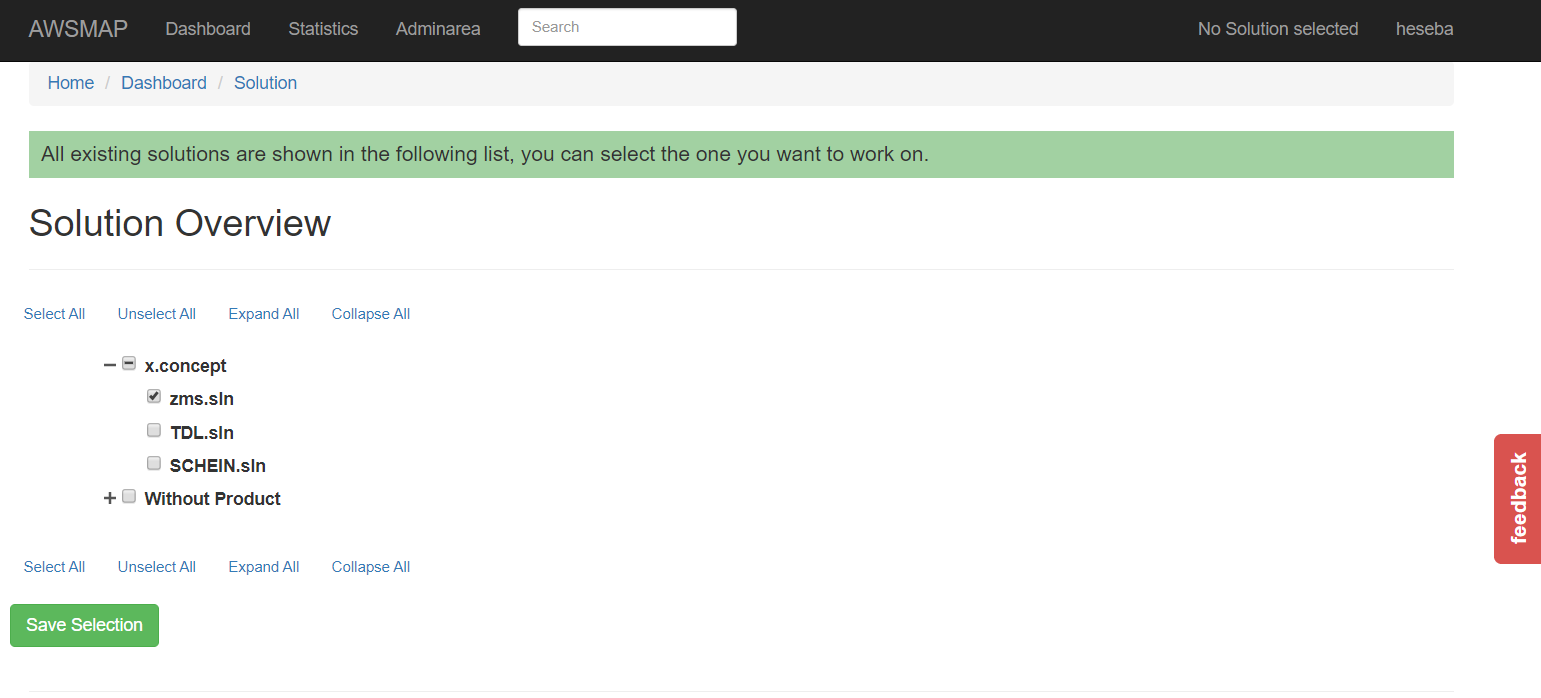
\includegraphics[width=0.99\textwidth]{../figures/screenshots/awsmap-solution-picker.png}
\caption[Solution Picker View]{Solution Picker View in medatixx Version of Annotation Platform}\label{fig:eval.awsmap}
}
\end{figure}\vspace{-20pt}

A fork of the Annotation Platform described in \cref{sec:extraction.platform} was created with specific adaptions to the environment of medatixx.
This version was deployed at medatixx and connected to its MS Team Foundation Server instance.
From this TFS, the codebase was loaded into the Annotation Platform through a dedicated batch import implementation created to accelerate loading of the large amount of software \glspl{artifact} contained in the production code.
Another adaption in the medatixx-specific fork of the Annotation Platform is the product/solution switcher.
It allows to temporarily limit the scope of the software \glspl{artifact} represented in the Annotation Platform to specific software products or MS Visual Studio solutions.
The medatixx instance of the Annotation Platform was tested by volunteers from the software development department and the software architect.
\Cref{fig:eval.awsmap} shows the solution picker view of the medatixx-specific version of the Annotation Platform.
The products and solutions listed can be used to filter the \glspl{artifact} shown in the Annotation Platform.
The red button on the right was implemented to support feedback, e.g. on bugs or feature requests, and keeps track of the viewing context in which the feedback was sent.
The logged-in user shown on the top right of the screen is authenticated against an Active Directory Domain controller.

\vspace{-10pt}
\subsection[Rapid Web Migration Prototyping of Medical \\ Appointment Scheduling]{Rapid Web Migration Prototyping of Medical Appointment Scheduling}
\vspace{10pt}

The testing of AWSM:RM was based on the medical appointment scheduling scenario described in \cref{sec:scenario-code}.
As outlined in \cref{tbl:legacy_characteristics}, it provides basic functionality for management of appointments in resident doctor's offices, including the creation, modification, deletion, and viewing of existing appointments in different calendar views and the search for free timeslots to allocate new appointments into.
To create a \gls{web migration prototype} of the core functionality of the scenario application, we applied the \gls{wasm}-based AWSM:RM business logic reuse technique, building a demonstrative prototype that provides calendar view, appointment entry and free timeslot search functionality executing \legacy business logic modified through and supported by the ReWaMP tool.
\Cref{fig:eval.rewamp} shows a screenshot of a \gls{web migration prototype}, featuring a calendar view with WASM-enabled business logic taken from the medical appointment scheduling scenario application.
\begin{figure}[t]
\hypertarget{fig:eval.rewamp}{%
\centering
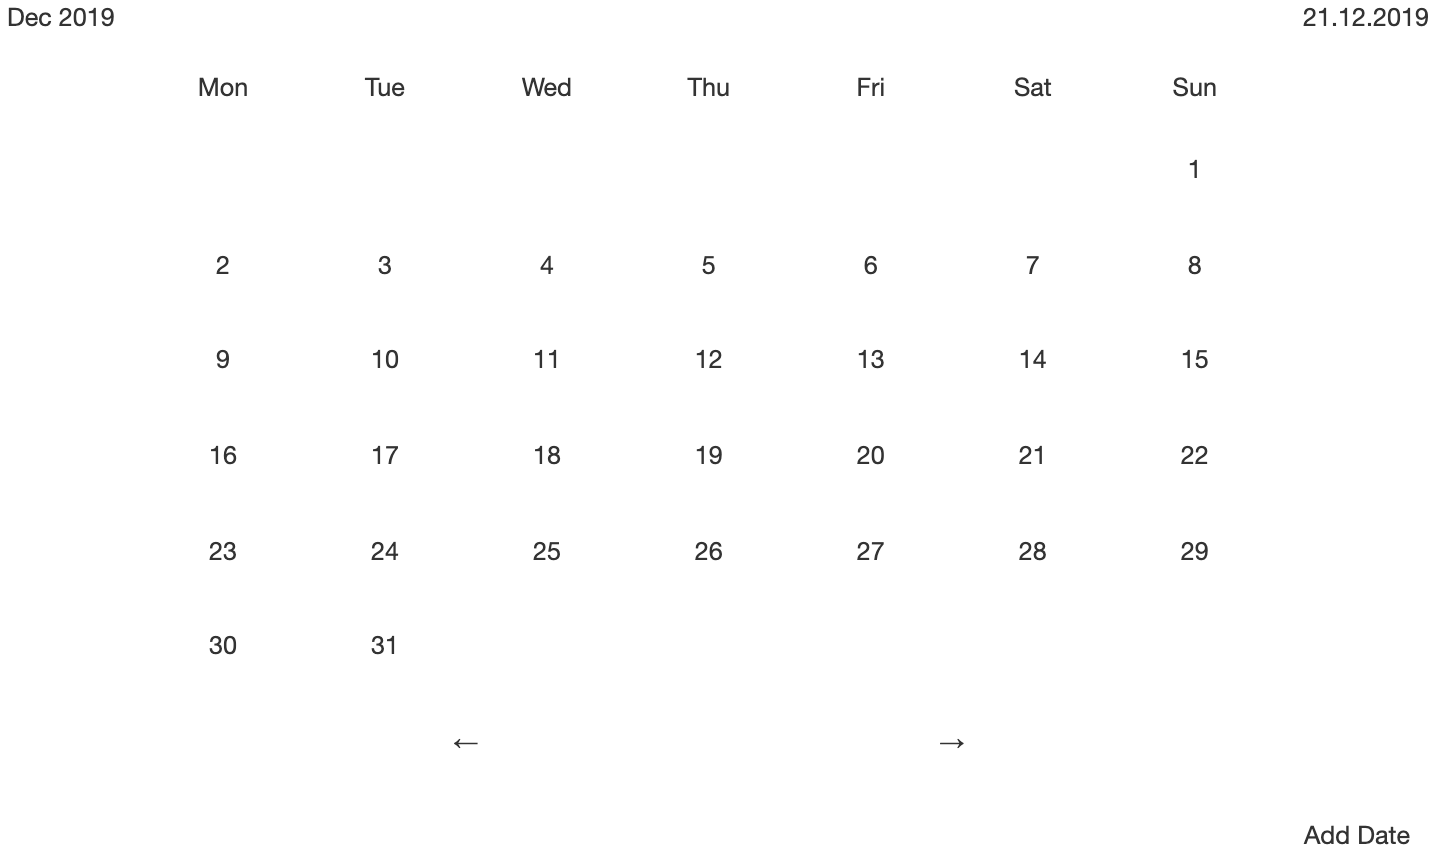
\includegraphics[width=0.75\textwidth]{../figures/screenshots/rewamp-calendar.png}
\caption[Calendar View of Web Migration Prototype]{Calendar View of Web Migration Prototype with \\ WASM-based Business Logic reused from Legacy System}\label{fig:eval.rewamp}
}
\end{figure}

The important characteristic of this prototype is the reuse of parts of the \legacy business logic.
As shown in the example in \cref{lst:rewampcpp} these parts are exported into JavaScript from the \cpp code, which is compiled to \gls{wasm} and then, as shown in \cref{lst:rewampjs} they can be bound in JavaScript to handle the click events in the \web user interface, redirecting to the compiled \gls{wasm} module.
\begin{lstlisting}[language=C++, captionpos=t, caption=Example of C++ Code Added by ReWaMP to Export Legacy Functionality to JavaScript, label=lst:rewampcpp]
EMSCRIPTEN_BINDINGS(rwmp_binds){
  using namespace emscripten;
  class_ <Cal01_View>("Cal01_View")
    .constructor()
    .function("OnOK", &Cal01_View::OnOK)
    .function("OnBnClickedButtonAdddate",
      &Cal01_View::OnBnClickedButtonAdddate);
}
\end{lstlisting}
\begin{lstlisting}[language=JavaScript, captionpos=t, caption=JavaScript Binding EventHandler of Button to Exported Legacy Functionality, label=lst:rewampjs]
function rwmp_init() {
  rwmp =  new Module.Cal01_View();
  rwmp.OnInitDialog();
  ...
  document.getElementById("IDC_BUTTON_ADDDATE")
    .addEventListener("click", function(){
      rwmp.OnBnClickedButtonAdddate();
  });
}
\end{lstlisting}


The UI Transformer tool was tested on MFC-based \legacy user interfaces from the scenario application to automatically create \web versions of the user interfaces.
Based on these \gls{ui} prototypes, additional CSS styling resulted in user interfaces like the calendar shown in \cref{fig:eval.ui-transform}.

\begin{figure}[h!]
\hypertarget{fig:eval.ui-transform}{%
\centering
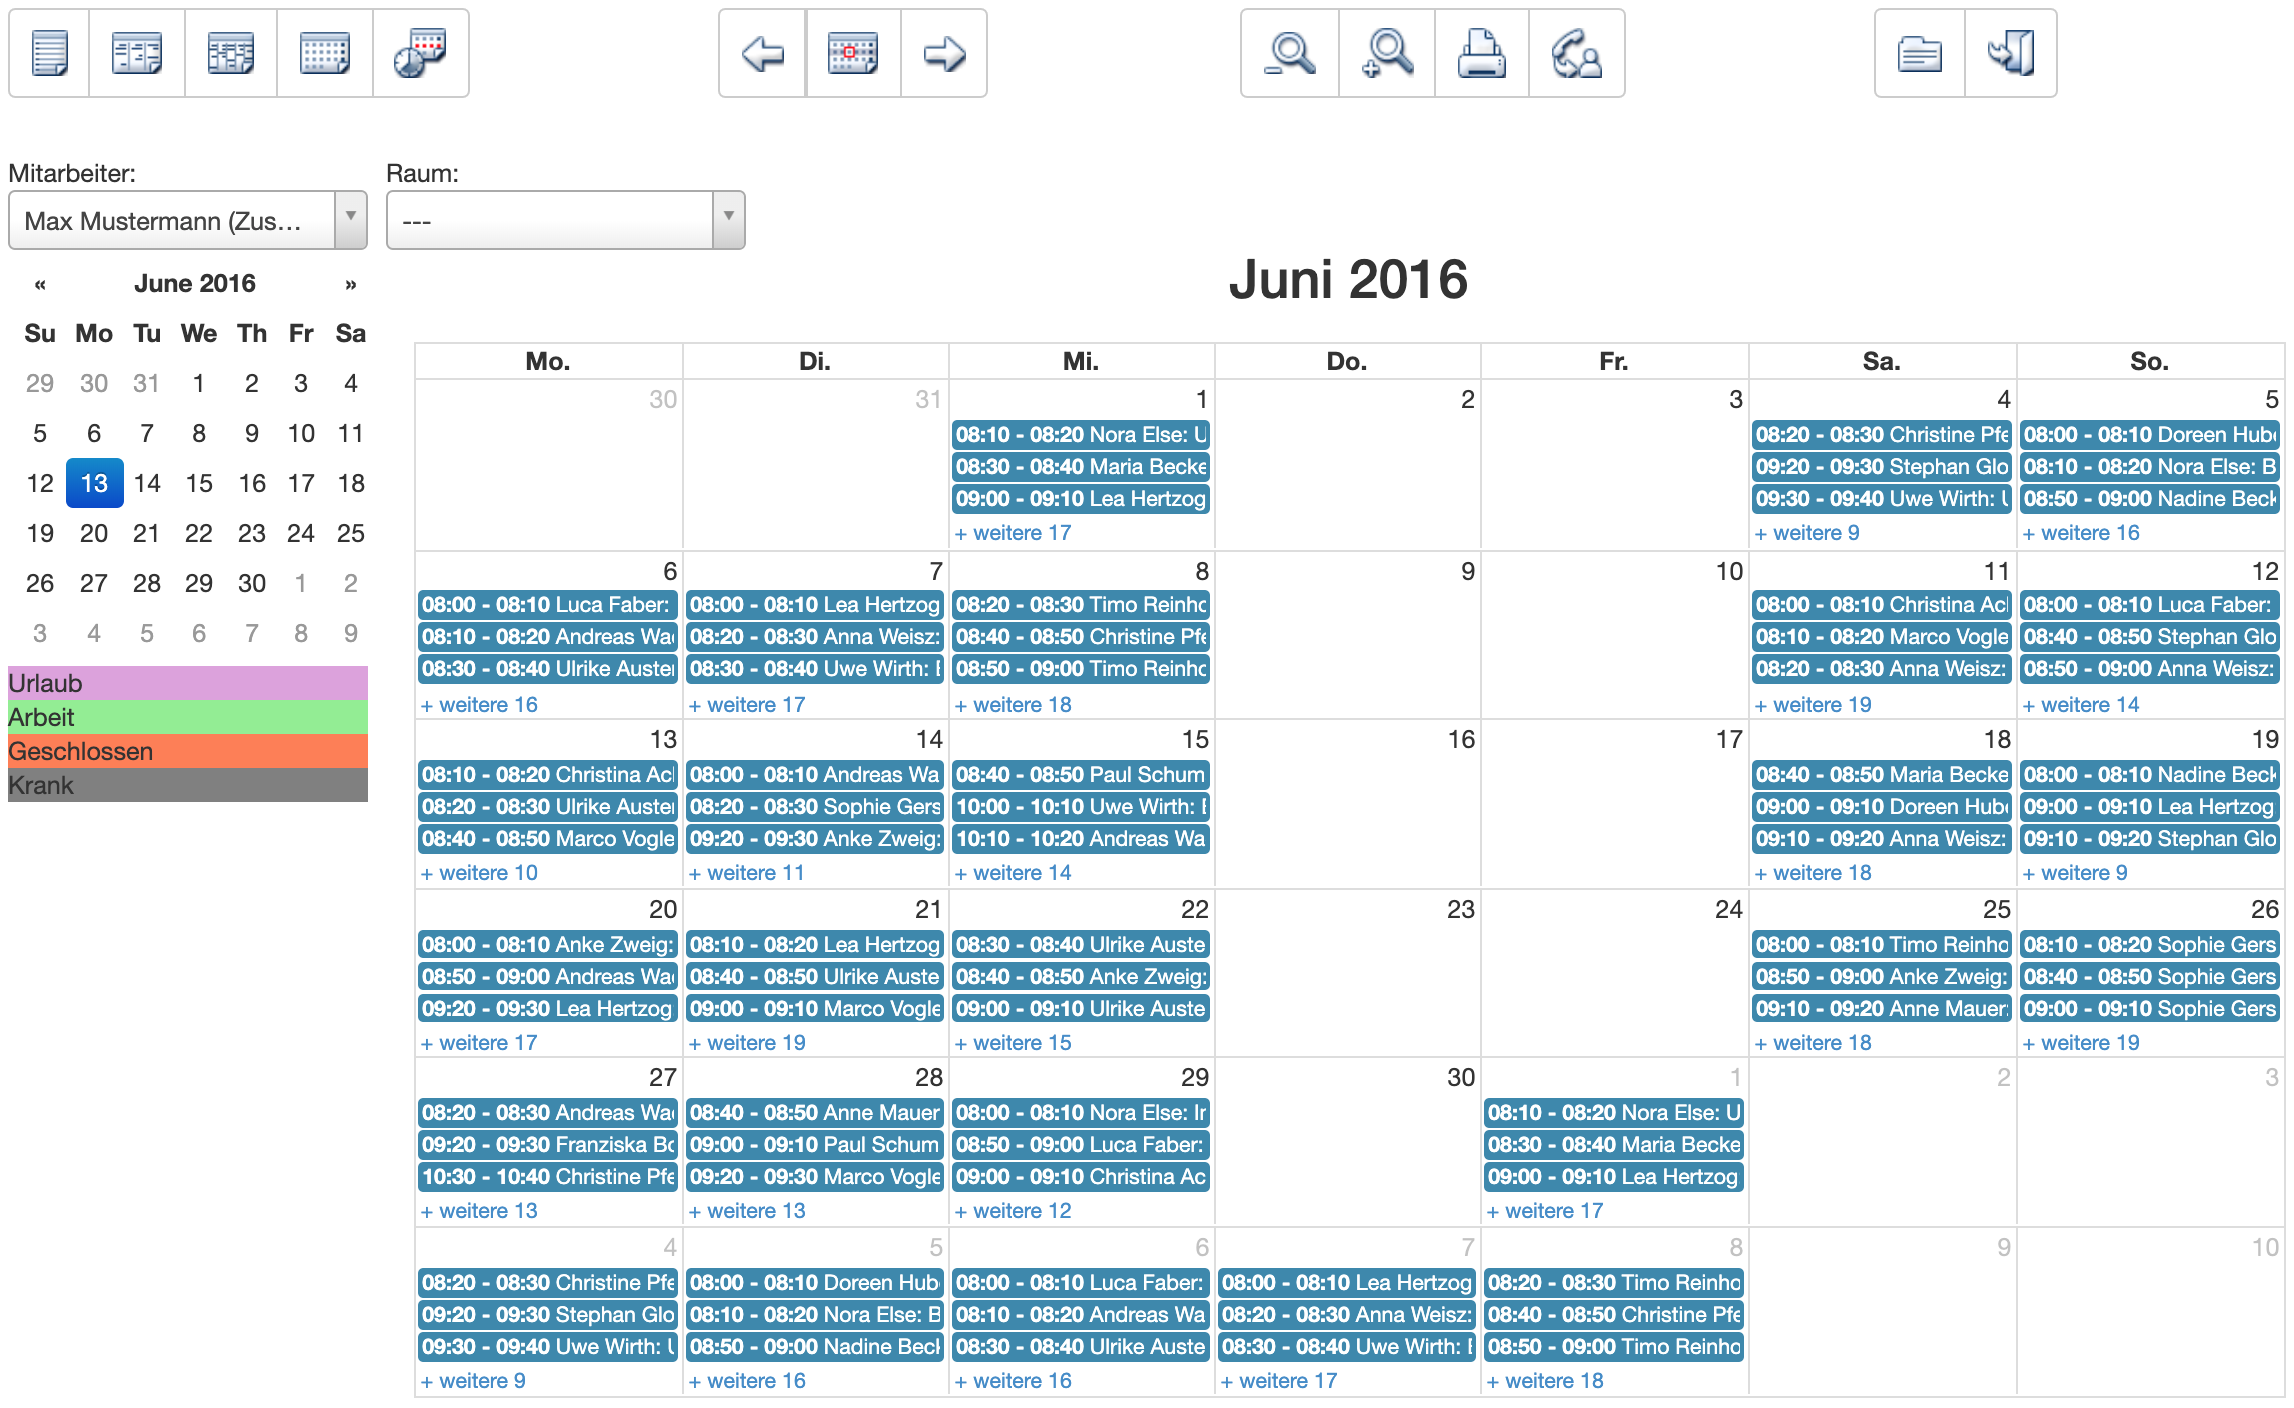
\includegraphics[width=0.9\textwidth]{../figures/screenshots/calendar.png}
\caption[Web Version of Calendar User Interface]{Web Version of Calendar User Interface of Scenario Application}\label{fig:eval.ui-transform}
}
\end{figure}

\subsection{Layout Similarity Measurement in x.concept}
\vspace{10pt}

\begin{figure}[h!]
\hypertarget{fig:eval.similarity}{%
\centering
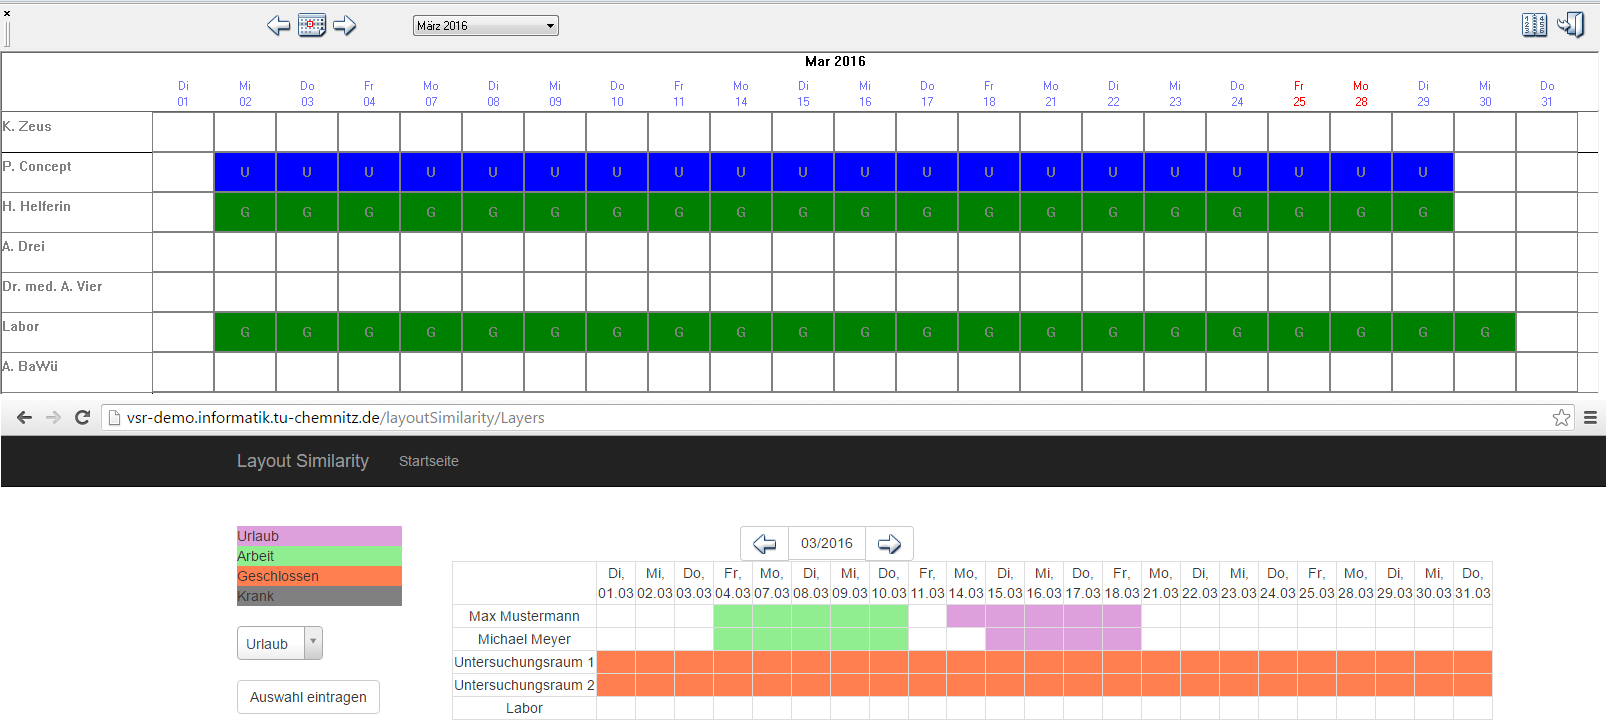
\includegraphics[width=0.9\textwidth]{../figures/zms.png}
\caption[ZMS Legacy and Web User Interfaces]{Legacy Desktop (top) and Web (bottom) user interface from ZMS, \\ used in Similarity Measurement Experiments}\label{fig:eval.similarity}
}
\end{figure}
The AWSM:CI Layout Similarity Measurement was tested on user interfaces of the medatixx x.concept Desktop application described in \cref{sec:scenario-code}.
For three different views -- a graphical shift schedule, a calendar view, and a patient data form -- \web versions of the user interfaces were systematically altered in layout dimensions as described in \cref{sec:calibration}.
The test subjects were acquainted with the original desktop user interfaces of x.concept and then evaluated the similarity with the different variations of their \web versions.
The results of this empirical experiment were compared with the objective similarity measures proposed in \cref{sec:computing-sim} to verify their applicability for comparisons of real \legacy user interfaces and their \web versions and to demonstrate the calibration process.
\Cref{fig:eval.similarity} shows the user interface of the graphical shift schedule.
The \legacy desktop user interface shown on top was analyzed comparatively against different \webbased versions like the one shown on the bottom, and the results of similarity computation were compared with empirical similarity evaluation results.

\vspace{-15pt}
\hypertarget{sec:evaluation.summary}{%
\section{Summary}\label{sec:evaluation.summary}}
\vspace{15pt}

While previous sections evaluated the \gls{awsm} Methods and techniques in isolation, this section analyzed the extent to which the \gls{awsm} Methodology and Toolsuite as a whole satisfy the requirements for a \gls{Web Migration} solution addressing the shortcomings of existing approaches as elicited in \cref{sec:sota.shortcomings}.
The analysis showed that all scope requirements and all stakeholder requirements except Expertise and Process Integration are fully satisfied.
The latter two requirements are partially satisfied acknowledging the specificity of \gls{Web Migration} and its activities, which cannot be conducted entirely without additional expertise requirements and completely integrated with ongoing development except for simple \gls{Encapsulation} approaches or approaches with limited scope.
The chapter has compared \gls{awsm} with the state of the art in the \gls{Web Migration} field, showing that \gls{awsm} Methods and tools successfully address gaps in existing comprehensive \gls{Web Migration} approaches.
A brief overview of application of \gls{awsm} techniques and tools in the context of the \gls{isv} scenario was given.
